Section~\ref{sec:related-work-fully-trustless} has already outlined the invariable need for clock synchronization, when it comes to reach progressively more accurate, correct, sound, and tamper-proof means of location attestation. What has not been discussed yet is the bridge between the clock synchronization problem and the consensus problem, in the specific context of distributed systems. 

This section will briefly discuss how these two fundamental problems are, in fact, intertwined. In simple terms, synchronizing clocks is nothing more profound than reaching agreement about the current time of the internal clocks of a distributed setting of machines. The indiscriminate case of clock synchronization can be stretched to a continued act of counting time at the same pace, as the indiscriminate case of reaching agreement about the current time of the internal clocks can be extended to a continued act of reaching agreement about the current state of the system. The latter is the consensus problem, and the former is a special case of it, the case of time synchronization. As argued in Section~\ref{sec:background-permissionless-consensus}, craving to achieve time synchronization, in not just a distributed setting, but in a fully trustless environment, can be transposed to the problem of achieving permissionless consensus, fulfilling the need for ordering and synchronizing events, at the same pace, in an environment where individual participants are not necessarily trusted. The first example depicted in Figure~\ref{fig:proof-of-location-example-scenarios} makes it clear that the eyewitnesses can only attest to the reporter's presence at the accident site if they had been there at the same time and witnessed the same event. However, these entities are not necessarily known to each other and to anyone else around, nor are they necessarily trusted. This implies not trusting that the clocks of the witnesses are correctly adjusted, as well. Therefore, the witnesses need to reach agreement about the current time, in order to be able to collectively and correctly attest to the reporter's presence at the accident site, in a given moment, otherwise they would all have conflicting or different reports. Additional to that, they may also attest to the reporter's course of action, by the means of taking pictures or recording videos, which are also events that may be ordered and synchronized, achieving, thus, permissionless consensus.

In consequence and specifically regarding the \pol{} problem, the need for clock synchronization is not only a matter of achieving more accurate positioning measures, as typically done in GPS-related trilateration systems, but a fundamental matter of achieving complete and sound consensus between the witnesses that are set to attest to one's location. Fundamentally, as defined in Section~\ref{sec:background-proof-of-location}, a \pol{} is complete if the attestation is done at location $l$ and time $t$, by a set of witnesses $w \in W$. To cope, as well, with the proposed property of spatio-temporal soundness, these witnesses should invariably reach consensus. They should not just agree to exist at around the same location $l$, relative to the precision, reliability, and coverage of their physical communication means, but should also agree on the time $t$, relative to the precision of their internal clocks. The latter is exactly the clock synchronization problem, folded into the greater and abstract need for consensus. The FOAM protocol proposes the achievement of such a time agreement with the employment of a self-stabilizing hybrid fault-tolerant clock synchronization protocol \cite{foam-white-paper, malekpour2015self}. The authors justify the choice highlighting the formal verification methods employed in Malekpour's work. This distributed algorithm is expected to formally work to the extent of the presence of a one third minority of Byzantine nodes \cite{lamport2019byzantine}. This fact validates the theoretical need for a composition of at least four witnesses for the most basic configuration of a zone, in the FOAM protocol. 

\begin{figure}[b!]
    \begin{center}
    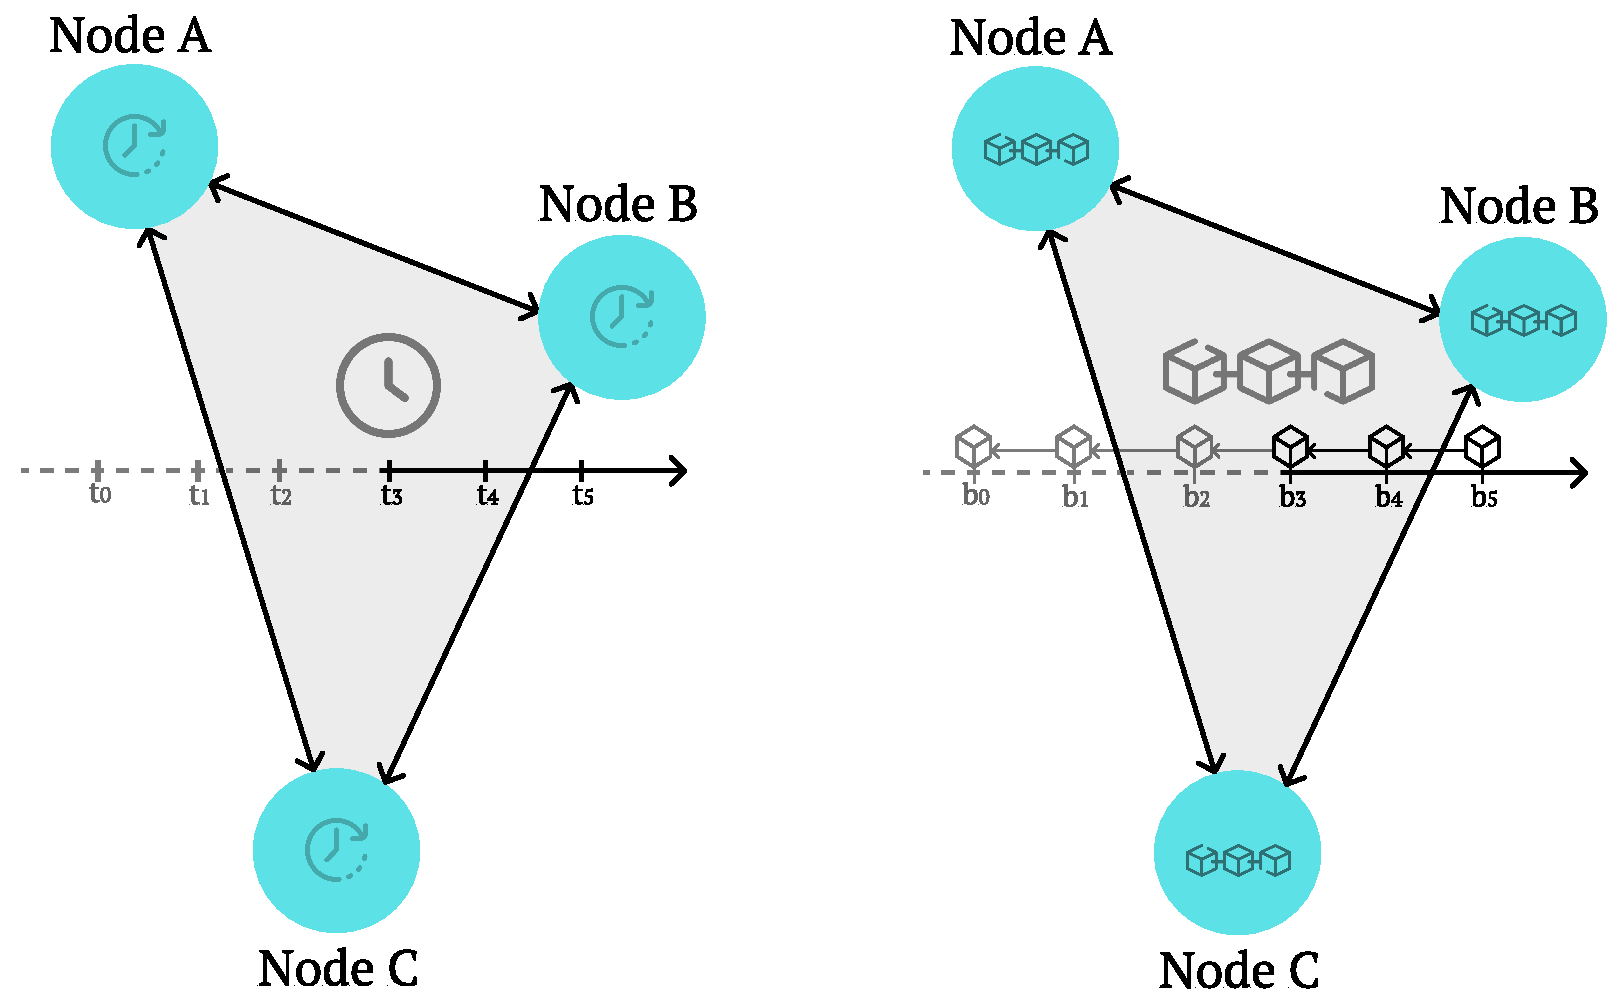
\includegraphics[width=0.8\textwidth]{overview-pol-time-sync.pdf}
    \caption{The goal of establishing zone-relative time consciousness, on the left, by the employment of a clock synchronization protocol, and on the right, by the employment of a consensus mechanism. Relative to the precision of both frequencies, the two mechanisms should achieve the same result, with the latter allowing for a strongly consistent serialization of transactions and total order of multidimensional information.}
    \vspace{-1cm}
    \label{fig:proof-of-location-overview-time-sync}
    \end{center}
\end{figure}

\begin{figure}[b!]
    \begin{center}
    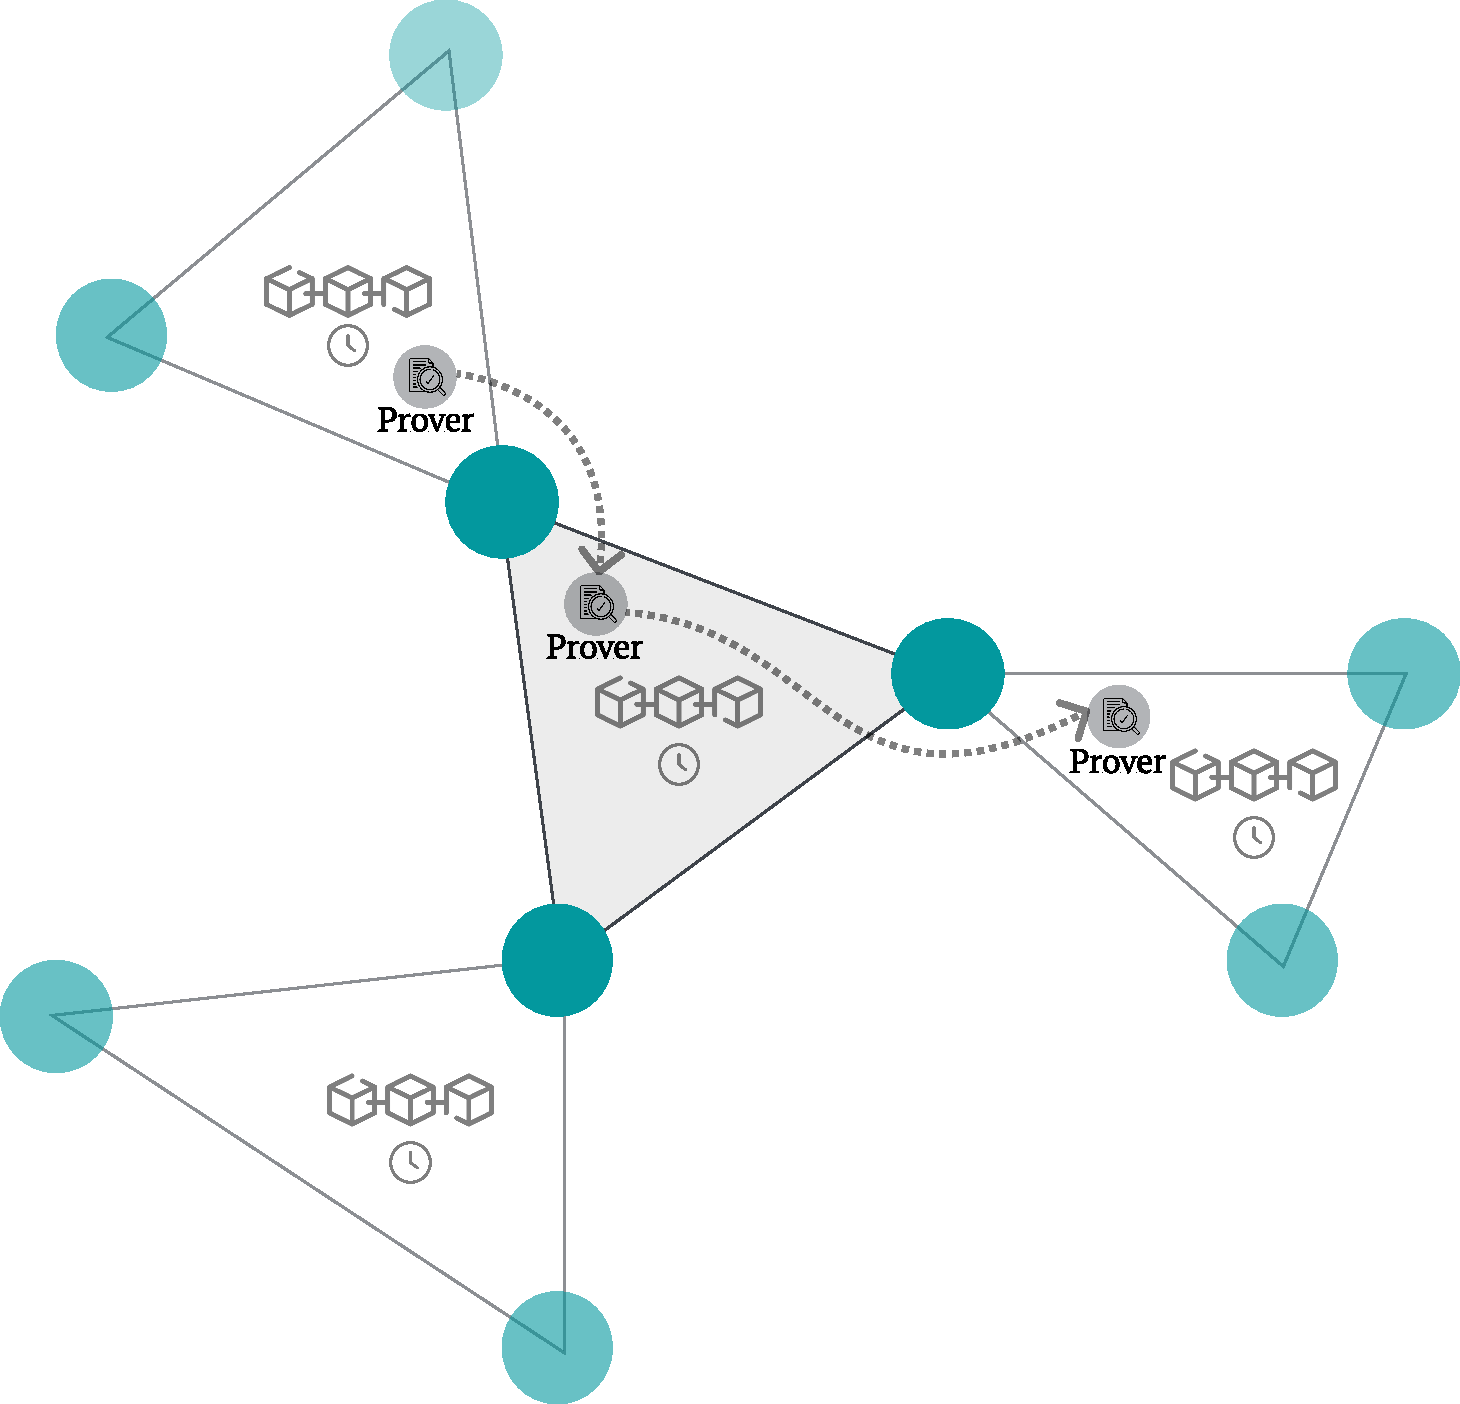
\includegraphics[width=0.6\textwidth]{overview-pol-latticework.pdf}
    \caption{The dense latticework of time-conscious witnessing zones, providing location services. Such a structure would allow for more accurate and verifiable location attestations, for example, regarding moving provers that constantly change their locations.}
    \vspace{-1cm}
    \label{fig:proof-of-location-overview-latticework}
    \end{center}
\end{figure}

This thesis proposes, instead, the empirical experimentation with a permissionless consensus mechanism, in the lines of the ones introduced in Section~\ref{sec:background-permissionless-consensus}. The goal, as illustrated in Figure~\ref{fig:proof-of-location-overview-time-sync}, is equivalent to establishing zone-relative time consciousness, but with the added benefit of providing strongly consistent serialization of transactions and total order of multidimensional events, instead of simply counting time in a unidimensional manner. The technicalities of modern systems that tackle the permissionless consensus problem allow, as well, for stronger guarantees in terms of security, tamper-proof and censorship resistance, as discussed in Section~\ref{sec:related-work-fully-trustless}. The fault-tolerance guarantees of a typical deterministic-finality Byzantine fault-tolerant algorithm are shifted back to a probabilistic finality fault-tolerance threshold, where the probability of a transaction being finalized is directly proportional to the number of nodes that have approved it \cite{survey-dist-consensus}. This is, arguably, a more desirable property for the considerations of a decentralized \pol{} protocol, where the finality of a location certificate is directly proportional to the number of witnesses that have seen the prover, and thus, the number of witnesses that have agreed on the time of the attestation, in the context of trustless environments. The methodical work of formally verifying, measuring, and comparing the two approaches, in the specific context of \pol{} protocols, is also left for future work. This thesis will plainly focus on the experimentation with a consensus mechanism that not only allows for the logical synchronization of clocks, via the regulation of the block interval, an inherent property of such mechanisms, but also for the achievement of a distributed and time-conscious Turing Complete environment, where the execution of more sophisticated logic is structurally enabled, in a decentralized setting. Another point worth mentioning is the extensibility of the proposed way of achieving clock synchronization, which should also be researched further, to assess the need and evaluate the possibility for independently calculating the geometry of the zone, and the practicability of trilateration mechanisms to more accurately determine the prover's exact location \cite{foam-white-paper}. Nevertheless, the approach aligns itself with the idea of a dense web of clocks, as depicted in Figure~\ref{fig:proof-of-location-overview-latticework}. The end goal for the coverage expansion of such a \pol{} protocol is to achieve a global latticework of witnessing zones that provide location services. This resonates with the faraway goal of achieving a secure, verifiable, decentralized, global, and consensus-driven map of the world \cite{king_2020,foam-white-paper}.

The potential Turing Completeness property of the envisioned consensus system fundamentally allows for a network of nodes to perform arbitrary computations in a decentralized and fault-tolerant manner. At its core and in more tangible terms, such a system allows for the creation of smart contracts, as self-executing code agreements that are dictated by the terms of the direct consensus between the entities that are involved in the \pol{} protocol. By using a distributed Turing-Complete system, these smart contracts can be deployed across the network, and their execution can be verified by all entities, ensuring that the terms of the contract are met \cite{buterin2014next}. This allows for the simple transactional case of registering a valid \pol{} claim by the prover, which will be covered in this thesis, and also for progressively more complex location claims. Pictured in Figure~\ref{fig:proof-of-location-overview-turing}, a Turing Complete system could, for example, attest to the simultaneous existence of a group of provers, or enforce a set of arbitrary terms dictated by the verifier, the witnesses, or by zone-specific requirements, among all other endless computable possibilities that one may envision. 

\begin{figure}[h!]
    \begin{center}
    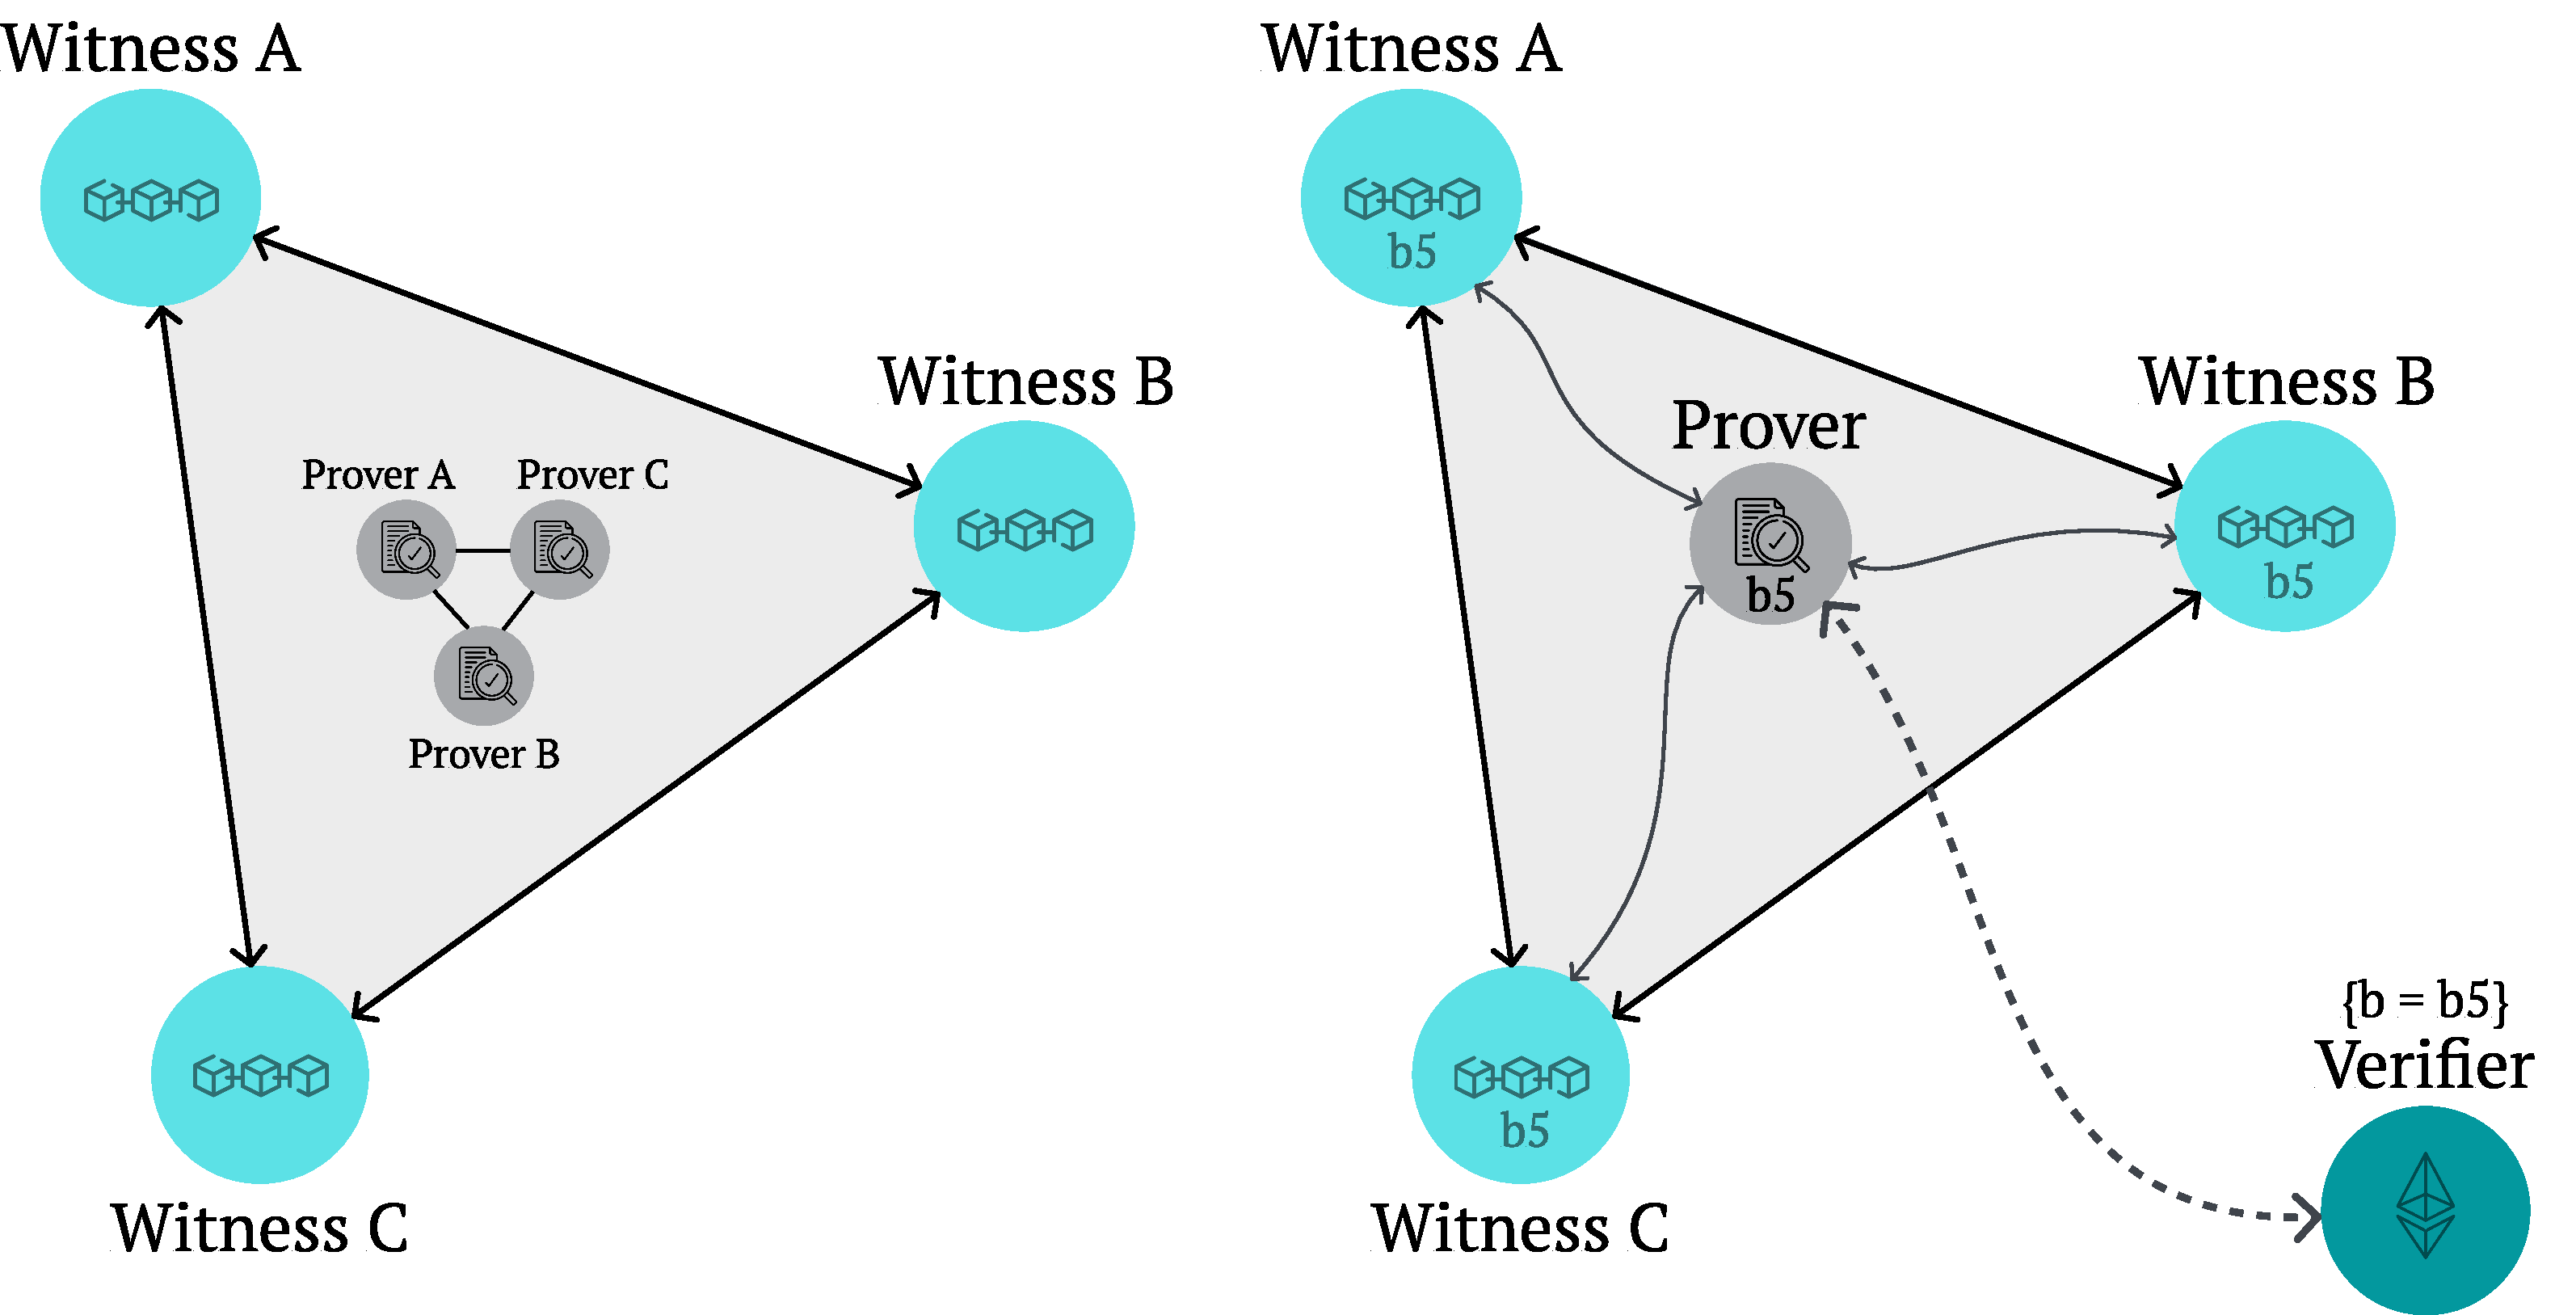
\includegraphics[width=0.9\textwidth]{overview-pol-turing.pdf}
    \caption{Some more sophisticated use cases of a Turing Complete \pol{} protocol, where the execution of zone-relative smart contracts is enabled. On the left, a multi-prover configuration, and on the right, the case where a verifier enforces the attestation of the prover's location at a specific block or time.}
    \vspace{-0.5cm}
    \label{fig:proof-of-location-overview-turing}
    \end{center}
\end{figure}

With all the above considerations in mind, this thesis is set to demonstrate the simplest case of the application of a consensus mechanism to achieve time synchronization. The goal is to experimentally prove that the block interval of a consensus mechanism can be used to synchronize  the clocks of a network of nodes, and thus, achieve zone-relative time consciousness. All the other considerations, like the extensibility of the proposed approach, the possibility of achieving a more accurate location attestation, or making use of the Turing Completeness of the system for more complex logic, are left for future work. The next section will cover the proof generation process to finally produce a \pol{} claim.